\documentclass[sigconf,nonacm]{acmart}
\usepackage[ngerman]{babel}
\usepackage{booktabs}
\usepackage{tabularx}
\usepackage{array}
\usepackage{enumitem}
\settopmatter{printacmref=false}
\renewcommand\footnotetextcopyrightpermission[1]{}
\newcolumntype{L}[1]{>{\raggedright\arraybackslash}p{#1}}
\newcolumntype{Y}{>{\raggedright\arraybackslash}X}
% Link zum Repository hier eintragen:
\newcommand{\repourl}{\url{https://github.com/Kolie11/projekt2-recybot-2}}

\begin{document}
\title{RecyBot 2.0: Konzeption und Pilotevaluation eines browserbasierten Lernspiels zu KI-Literacy und Kreislaufwirtschaft in der Sekundarstufe}

\author{Fassou Mathias Kolie}
\affiliation{\institution{Hochschule Ruhr West}\city{Bottrop}\country{Deutschland}}
\author{Daniil Gurin}
\affiliation{\institution{Hochschule Ruhr West}\city{Bottrop}\country{Deutschland}}

\begin{abstract}
KI-Literacy und Bildung für eine Kreislaufwirtschaft werden in Forschung und Lernangeboten bislang weitgehend getrennt behandelt. Wir untersuchen, wie ein Lernspiel gestaltet werden kann, das beide Themen für Lernende der Sekundarstufe in einem zusammenhängenden Lernkonzept verbindet, und welche Lernwirkung es in einer ersten Erprobung zeigt. Im Sinne von Design-Based Research leiten wir aus Kompetenzrahmen, Lerntheorien und einem Vergleich mit vier Referenzsystemen neun Gestaltungsanforderungen ab, wählen Lernziele anhand offengelegter Kriterien aus und ordnen Lern- und Spielmechaniken mit dem LM-GM-Modell zu. Das Ergebnis, RecyBot 2.0, ist ein browserbasiertes Lernspiel mit neun Modulen entlang des Stoffkreislaufs einer fiktiven Stadt, in denen Lernende echte KI-Modelle trainieren. Eine explorative Pilotstudie mit $N = 11$ Erwachsenen (Prä-/Post-Wissenstest, System Usability Scale) ergab einen Zuwachs mittlerer Effektstärke ($d_z = 0.67$), der statistisch nicht signifikant war ($p = .052$), sowie eine verbesserungsbedürftige Usability (SUS $= 57.7$). Wir diskutieren Gestaltungsimplikationen und leiten Änderungen für den nächsten Entwicklungszyklus ab. Anwendung, Quellcode, Erhebungsmaterialien, Rohdaten und Auswertungsskript sind offen verfügbar.
\end{abstract}

\keywords{KI-Literacy, Kreislaufwirtschaft, Game-Based Learning, Serious Games, Design-Based Research, Sekundarstufe}

\begin{teaserfigure}
\centering
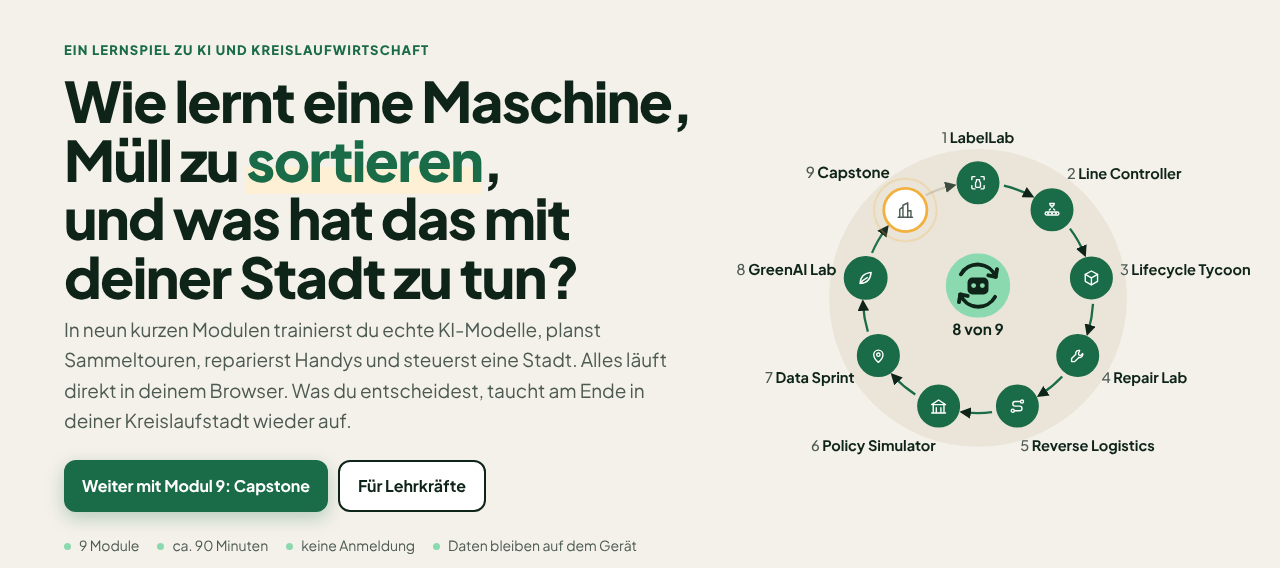
\includegraphics[width=0.92\textwidth]{fig/fig_hub.png}
\caption{Startseite von RecyBot 2.0: Die neun Module sind als Stationen eines Stoffkreislaufs angeordnet.}
\Description{Bildschirmfoto der Startseite mit einer kreisförmigen Anordnung der neun Module.}
\label{fig:hub}
\end{teaserfigure}

\maketitle

\section{Einleitung}
Künstliche Intelligenz (KI) ist Teil alltäglicher Infrastruktur, häufig ohne sichtbar zu sein. In Sortieranlagen für Verpackungsabfälle entscheiden etwa Kameras und Nahinfrarot-Sensoren gemeinsam mit Klassifikationsmodellen, welcher Gegenstand auf welchem Band landet. Zugleich ist die Kreislaufwirtschaft (Circular Economy, CE) ein zentrales umweltpolitisches Ziel: Produkte sollen langlebig, reparierbar und recycelbar sein, und Abfall soll möglichst nicht entstehen \cite{emf2013,eu2020}.

Für Schüler:innen sind beide Themen bildungsrelevant. Die KMK fordert, dass Lernende digitale Systeme verstehen und ihre Auswirkungen beurteilen können \cite{kmk2016}; Nachhaltigkeitsbildung zielt auf Kompetenzen wie Systemdenken \cite{wiek2011}. Kompetenzrahmen zur KI-Literacy \cite{long2020,touretzky2019,unesco2024} und Lernangebote, in denen Lernende eigene Modelle trainieren \cite{carney2020,lane2021,codeorg2019}, behandeln Anwendungsfelder jedoch meist nur als Kulisse, während Lernspiele zur Kreislaufwirtschaft ohne KI auskommen und sich überwiegend an Studierende richten \cite{lange2022}. Dabei erklären sich beide Themen gegenseitig: Eine Sortier-KI ist nur so gut wie ihre Trainingsdaten, und ein Produkt aus untrennbarem Verbundmaterial kann auch die beste KI nicht recyceln.

Daraus ergeben sich drei Forschungsfragen:

\begin{description}[leftmargin=2.4em,labelwidth=2em,labelsep=0.4em,itemsep=2pt]
\item[FF1] Wie lassen sich Lernziele, Inhalte und Spielmechaniken eines Lernspiels, das KI-Literacy und Kreislaufwirtschaft verbindet, nachvollziehbar aus Kompetenzrahmen, Lerntheorien und Referenzsystemen ableiten?
\item[FF2] Zeigt sich nach der Nutzung des Spiels ein Zuwachs an konzeptuellem Wissen?
\item[FF3] Wie wird die Usability bewertet, und welcher Über\-arbeitungs\-bedarf ergibt sich?
\end{description}

Der Beitrag der Arbeit ist dreifach: (1) eine offengelegte Ableitung von Anforderungen, Lernzielen und Spielmechaniken (Abschnitt~\ref{sec:design}), (2) die quelloffene Webanwendung RecyBot 2.0 und (3) eine explorative Pilotstudie mit offen verfügbaren Daten und Materialien (Abschnitte~\ref{sec:method}--\ref{sec:discussion}). FF1 wird durch den Gestaltungsprozess beantwortet, FF2 und FF3 durch die Pilotstudie.

\section{Verwandte Arbeiten}
\label{sec:related}
\subsection{KI-Literacy in der Schule}
Long und Magerko definieren KI-Literacy als Kompetenzen, KI kritisch zu bewerten, mit ihr zu kommunizieren und sie als Werkzeug zu nutzen, und beschreiben 17 Kompetenzen entlang von fünf Leitfragen \cite{long2020}. Die AI4K12-Initiative formuliert fünf „Big Ideas“ für den Schulunterricht \cite{touretzky2019}; der UNESCO-Kompetenzrahmen ordnet zwölf Kompetenzen vier Dimensionen und den Niveaus Verstehen, Anwenden und Gestalten zu \cite{unesco2024}. Übereinstimmend wird empfohlen, KI nicht nur zu erklären, sondern selbst auszuprobieren: Das eigene Trainieren von Modellen unterstützt das Verständnis ihrer Funktionsweise \cite{druga2019}, und interaktives maschinelles Lernen macht Modellverhalten für Laien nachvollziehbar \cite{amershi2014}.

\subsection{Spielerisches Lernen zur Kreislaufwirtschaft}
Kreislaufwirtschaft wird in Definitionen häufig auf „Reduce, Reuse, Recycle“ verkürzt, während die systemische Perspektive selten explizit ist \cite{kirchherr2017}. Zentrale Gestaltungsstrategien sind Langlebigkeit, Reparierbarkeit und Zerlegbarkeit \cite{bocken2016} sowie der Werterhalt durch Reparatur vor dem Recycling \cite{stahel2013}. Spielerische Ansätze adressieren vor allem die Systemsicht, etwa das Brettspiel Re-organise zur Innovation zirkulärer Geschäftsmodelle für Studierende \cite{lange2022}.

\subsection{Lernwirksamkeit von Lernspielen}
Game-Based Learning spricht kognitive, motivationale, emotionale und soziale Prozesse an \cite{plass2015}. Lernspiele wirken vor allem, wenn sie aktives Problemlösen erfordern, direktes Feedback geben und die Komplexität schrittweise steigern \cite{mayer2019}. Serious Games sind konventionellem Unterricht überlegen, besonders wenn sie mit weiterer Instruktion kombiniert und in mehreren Sitzungen genutzt werden \cite{wouters2013}; eine durchgehende Handlung kann das Engagement steigern, ohne den Lernerfolg zu mindern \cite{rowe2011}. Rein extrinsische Elemente wie Ranglisten können die intrinsische Motivation dagegen senken \cite{hanus2015}. Feedback gehört zu den wirksamsten Einflussfaktoren auf Lernleistung, besonders aufgabenbezogenes Feedback mit Hinweisen zum weiteren Vorgehen \cite{hattie2007,shute2008}, während rein entdeckendes Lernen ohne Anleitung Noviz:innen überfordert \cite{kirschner2006}.

\subsection{Referenzsysteme und Forschungslücke}
Tabelle~\ref{tab:ref} vergleicht vier Angebote, die jeweils einen Teil des Anspruchs abdecken. Teachable Machine \cite{carney2020}, Machine Learning for Kids \cite{lane2021} und AI for Oceans \cite{codeorg2019} lassen Lernende eigene Modelle trainieren und die Folgen ihrer Trainingsdaten erleben, beschränken sich aber auf Klassifikation und behandeln Anwendungsfelder höchstens als Kontext. Re-organise \cite{lange2022} vermittelt Systemzusammenhänge der Kreislaufwirtschaft, jedoch ohne KI und für Studierende. Uns ist kein Lernangebot bekannt, das KI-Literacy und Kreislaufwirtschaft für die Sekundarstufe so verbindet, dass Entscheidungen über KI und über den Stoffkreislauf aufeinander wirken.

\begin{table*}[t]
\caption{Vergleich von RecyBot 2.0 mit Referenzsystemen}
\label{tab:ref}
\small
\begin{tabularx}{\textwidth}{@{}L{3.3cm} L{2.4cm} L{3.2cm} L{2.6cm} Y L{2.5cm}@{}}
\toprule
\textbf{System} & \textbf{Zielgruppe} & \textbf{Eigenes Trainieren von KI} & \textbf{KI-Inhalte} & \textbf{Bezug zur Kreislaufwirtschaft} & \textbf{Format}\\
\midrule
Teachable Machine \cite{carney2020} & allgemein & ja (Bild, Ton, Pose) & Klassifikation & keiner & Web-Werkzeug ohne Spielrahmen\\
Machine Learning for Kids \cite{lane2021} & Kinder, Jugendliche & ja (Text, Bild, Zahlen) & Klassifikation & keiner & Projekte mit Programmierung\\
AI for Oceans \cite{codeorg2019} & ab Klasse 3 & ja (Labeln von Beispielen) & Trainingsdaten, Bias & Meeresmüll als Kontext, keine CE-Konzepte & Online-Aktivität, ca.\ 1 Stunde\\
Re-organise \cite{lange2022} & Studierende & nein & keine & zirkuläre Geschäftsmodelle, Systemsicht & Brettspiel\\
\midrule
\textbf{RecyBot 2.0} & Sekundarstufe I und II & ja (Bild, Entscheidungsbaum, neuronales Netz) & Trainingsdaten, Schwellwerte, Bias, Heuristiken, Energieverbrauch & Design, Reparatur, Sammlung, Sortierung, Politik, Systemsicht & Browser-Lernspiel, 90 Minuten\\
\bottomrule
\end{tabularx}
\end{table*}
\section{Methodisches Vorgehen}
\label{sec:approach}
Die Arbeit folgt dem Ansatz des Design-Based Research (DBR), der die Gestaltung einer Lernumgebung mit ihrer Erforschung in iterativen Zyklen aus Analyse, Gestaltung, Erprobung und Überarbeitung verbindet \cite{dbrc2003}. Dieses Paper dokumentiert den ersten Zyklus:

\begin{enumerate}
\item \textbf{Analyse:} narrative, konzeptgeleitete Literaturübersicht und Vergleich von Referenzsystemen (Abschnitt~\ref{sec:related}). Gesucht wurde in Google Scholar, der ACM Digital Library und IEEE Xplore mit Kombinationen der Begriffe \textit{game-based learning, serious games, AI literacy, AI education K-12, circular economy education, formative feedback} und \textit{cognitive load}, ergänzt durch Rückwärtssuche. Eingeschlossen wurden begutachtete Beiträge und etablierte Grundlagenwerke mit Bezug zu Lernen und Lehre, die auf schulische Lernende übertragbar sind; ausgeschlossen wurden rein technische Arbeiten ohne Bildungsbezug, außer als fachliche Grundlage einzelner Module. Trefferzahlen wurden nicht dokumentiert.
\item \textbf{Gestaltung:} Ableitung von Anforderungen, kriteriengeleitete Auswahl der Lernziele und Zuordnung von Lern- und Spielmechaniken mit dem LM-GM-Modell \cite{arnab2015} (Abschnitt~\ref{sec:design}).
\item \textbf{Erprobung:} explorative Pilotstudie mit Prä-/Post-Wissenstest und Usability-Messung (Abschnitte~\ref{sec:method} und \ref{sec:results}).
\item \textbf{Reflexion:} Ableitung von Änderungen für den nächsten Zyklus (Abschnitt~\ref{sec:discussion}).
\end{enumerate}

\section{Gestaltung von RecyBot 2.0}
\label{sec:design}
\subsection{Anforderungen}
Aus der Analyse ergeben sich neun Anforderungen, auf die sich alle Gestaltungsentscheidungen beziehen (Tabelle~\ref{tab:req}).

\begin{table}[t]
\caption{Aus Literatur und Referenzsystemen abgeleitete Anforderungen}
\label{tab:req}
\small
\begin{tabularx}{\columnwidth}{@{}L{0.55cm} Y L{1.9cm}@{}}
\toprule
\textbf{Nr.} & \textbf{Anforderung} & \textbf{Quelle}\\
\midrule
A1 & Handlungsorientierung: Lernende trainieren und testen echte Modelle selbst & \cite{long2020,druga2019}\\
A2 & Inhaltlich verankerte Spielmechanik; Belohnungen sparsam und an Lernziele gebunden & \cite{plass2015,hanus2015}\\
A3 & Unmittelbares, erklärendes Feedback & \cite{hattie2007,shute2008}\\
A4 & Angeleitete Exploration mit begrenzten Aufgaben und Erklärungen auf Abruf & \cite{kirschner2006}\\
A5 & Gestufte Komplexität von Einzelentscheidungen zu Systemen & \cite{sweller1988,paas2010}\\
A6 & Systemische Perspektive auf die Kreislaufwirtschaft & \cite{kirchherr2017,wiek2011}\\
A7 & Authentischer Kontext, an dem Wissen verankert wird & \cite{ctgv1990}\\
A8 & Verbindung von KI und Kreislaufwirtschaft (Lücke der Referenzsysteme) & Tab.~\ref{tab:ref}\\
A9 & Schulische Einsetzbarkeit: eine Doppelstunde, ohne Anmeldung und Programmierung, datensparsam & \cite{kmk2016}\\
\bottomrule
\end{tabularx}
\end{table}

\subsection{Auswahl der Lernziele}
Die Lernziele werden aus vier Kompetenzrahmen ausgewählt \cite{long2020,touretzky2019,unesco2024,wiek2011}, ergänzt um CE-Gestaltungsstrategien \cite{bocken2016,stahel2013}. Ein Element wird aufgenommen, wenn es vier Kriterien erfüllt: \textbf{K1 Kontextbezug} (an der Abfallwirtschaft mit der CE verbindbar; A7, A8), \textbf{K2 Erfahrbarkeit} (durch eigenes Handeln im Spiel erfahrbar; A1, A2), \textbf{K3 Machbarkeit} (ohne Programmierung in einer Doppelstunde erreichbar; A9) und \textbf{K4 Überprüfbarkeit} (Erreichen messbar). Tabelle~\ref{tab:lz} dokumentiert die Entscheidungen einschließlich der bewusst nicht aufgenommenen Elemente.

\begin{table*}[t]
\caption{Herleitung der Lernziele aus Kompetenzrahmen anhand der Kriterien K1--K4}
\label{tab:lz}
\small
\begin{tabularx}{\textwidth}{@{}L{3.2cm} L{4.6cm} L{2.2cm} Y@{}}
\toprule
\textbf{Rahmen} & \textbf{Element} & \textbf{Entscheidung} & \textbf{Begründung}\\
\midrule
Long \& Magerko \cite{long2020} & Wie funktioniert KI?; Was kann KI?; Wie sollte KI eingesetzt werden? & LZ1, LZ2, LZ4 & K1--K4 erfüllt: Lernen aus Daten, Fehlertypen, Bias und Zielsetzung sind handelnd erfahrbar\\
 & Was ist KI? & im Kontext & Voraussetzung, am Beispiel der Sortieranlage mitvermittelt\\
 & Wie nehmen Menschen KI wahr? & nicht aufgen. & K2, K4: kaum handelnd erfahrbar, schwer überprüfbar\\
AI4K12 \cite{touretzky2019} & Learning; Representation \& Reasoning; Societal Impact & LZ1, LZ2, LZ4 & Trainingsdaten, Entscheidungsbaum, Suche, Bias\\
 & Perception / Natural Interaction & Mittel / nicht aufgen. & Bilderkennung als Werkzeug; Sprachinteraktion ohne Bezug zur Abfallwirtschaft (K1)\\
UNESCO \cite{unesco2024} & Niveaus Verstehen und Anwenden & LZ1, LZ2, LZ4 & in 90 Minuten für die Zielgruppe erreichbar\\
 & Niveau Gestalten (KI-Werkzeuge erstellen) & nicht aufgen. & K3: erfordert Programmierung und mehr Zeit\\
Wiek et al.\ \cite{wiek2011} & Systemdenken; antizipatorische, normative und strategische Kompetenz & LZ3, LZ4 & Verzögerungen, Nebenwirkungen, Zielgewichtung, Gestaltungsentscheidungen\\
 & Interpersonale Kompetenz & nicht aufgen. & überwiegend Einzelspiel\\
CE-Strategien \cite{bocken2016,stahel2013} & Design, Reparatur, Rückführung & LZ3 & handelnd erfahrbar, Kern der CE jenseits des Recyclings\\
 & Geschäftsmodelle & nicht aufgen. & für die Sekundarstufe zu abstrakt (K1, K3)\\
\bottomrule
\end{tabularx}
\end{table*}

Die aufgenommenen Elemente werden zu vier Lernzielen gebündelt, nach der überarbeiteten Bloom-Taxonomie formuliert \cite{anderson2001} und von Verstehen zu Analysieren gestuft (A5):
\textbf{LZ1 Daten und Lernen:} erklären, wie Qualität und Vielfalt von Trainingsdaten das Verhalten einer KI bestimmen (Verstehen).
\textbf{LZ2 Entscheidungen von KI bewerten:} KI-Ausgaben als Wahrscheinlichkeiten deuten und Zielkonflikte wie Precision vs.\ Recall oder Genauigkeit vs.\ Energie abwägen (Anwenden, Bewerten).
\textbf{LZ3 Kreislaufprinzipien anwenden:} kreislauffähiges Design, Reparatur vor Recycling und effiziente Rückführung anwenden und begründen (Anwenden).
\textbf{LZ4 Systeme und Verantwortung:} Wechselwirkungen und Verzögerungen in einem Kreislaufsystem analysieren und begründen, wo Menschen Ziele für KI festlegen müssen (Analysieren).
LZ1 und LZ2 betreffen die KI im Kreislauf, LZ3 den Kreislauf selbst und LZ4 das Zusammenwirken beider.

\subsection{Didaktischer Rahmen}
Drei Theorien bilden das Gerüst, weil sie sich ergänzen. \textit{Experiential Learning} beschreibt Lernen als Zyklus aus Erfahrung, Reflexion, Begriffsbildung und Experimentieren \cite{kolb1984}; jedes Modul bildet ihn ab, wobei die Exploration durch klare Aufgaben und eingebaute Erklärungen begrenzt wird, da reines Erfahrungslernen Noviz:innen überfordern kann \cite{kirschner2006}. Die \textit{Cognitive Load Theory} \cite{sweller1988,paas2010} begründet die Stufung von Einzelentscheidungen (Module 1--4) zu Systemen (Module 5--9) und die Reduktion extrinsischer Belastung durch visuelle Darstellungen \cite{mayer2009}, ein Glossar und eine Vorlesefunktion. \textit{Constructive Alignment} \cite{biggs2011} verknüpft Lernziele (ILO), Spielmechaniken als Lernaktivitäten (TLA) und In-Game-Metriken, Vor- und Nachtest sowie ein Transfer-Quiz als Überprüfung (AT; Tabelle~\ref{tab:lmgm}). Motivationstheorien wie die Selbstbestimmungstheorie wurden nicht als eigenes Gerüst gewählt, da RecyBot vorrangig auf Wissenserwerb zielt; motivationale Aspekte fließen über die Gestaltung der Spielelemente ein \cite{hanus2015,vanroy2019}.

\subsection{Kontext und Material}
\textit{Abfallwirtschaft als Kontext:} Sie ist Teil der Lebenswelt aller Lernenden (A7), KI wird dort real eingesetzt, etwa in kamerabasierten und Nahinfrarot-Sortieranlagen (A1), und sie ist ein Kernbereich der Kreislaufwirtschaft (A8). Kontexte wie Verkehr oder Medizin würden KI ähnlich gut, die Kreislaufwirtschaft aber nur am Rand abbilden.
\textit{Fiktive Stadt:} „Grünstadt“ vereint alle Stationen des Kreislaufs in einem überschaubaren System, in dem Ursachen und Wirkungen kontrolliert modelliert werden können (A5, A6), und dient im Sinne der Anchored Instruction als gemeinsamer Anker aller Module \cite{ctgv1990}.
\textit{Objekte:} Sie erfüllen drei Kriterien: Alltagsnähe, eindeutige Zuordnung zu einem Lernziel und Bezug zu realen Verfahren. PET-Flaschen sind über das Pfandsystem bekannt und ein typisches Zielmaterial realer Sortieranlagen; am Wasserkocher lassen sich Material, Verbindungsart und Modularität mit je drei Ausprägungen überschaubar variieren (A5); am Smartphone werden Reparatur und Elektroschrott unmittelbar erlebbar.
\textit{Echte statt simulierter KI:} Wo möglich, werden echte Modelle im Browser trainiert oder ausgeführt (A1). Simuliert werden nur Größen, die im Klassenraum nicht real erzeugt werden können: Sensordaten und Energieverbrauch (Modul~8) sowie die Kennzahlen der Stadt (Modul~9).
\subsection{Gestaltungsprinzipien und Module}
Mit dem LM-GM-Modell \cite{arnab2015} wurde für jedes Modul festgelegt, welche Lernmechanik durch welche Spielmechanik umgesetzt wird und woran das Erreichen gemessen wird (Tabelle~\ref{tab:lmgm}). Modulübergreifend leiten sich daraus sechs Gestaltungsprinzipien ab, die über RecyBot hinaus auf Lernspiele zur KI-Literacy übertragbar sind.

\textbf{G1 Das KI-Konzept ist die Spielhandlung} (A1, A2). Lernende labeln Daten, setzen Schwellwerte oder trainieren Netze selbst, statt darüber zu lesen. Weil die KI falsche Labels unmittelbar übernimmt, werden frühe Datenfehler, die sich in realen Systemen durch alle späteren Schritte ziehen \cite{sambasivan2021}, direkt sichtbar; interaktives Lernen macht das Modellverhalten nachvollziehbar \cite{amershi2014}.

\textbf{G2 Fachliche Kennzahlen als Feedback} (A3). Statt eines Punktestands erhalten Lernende die Kennzahlen, mit denen auch Fachleute arbeiten: eine Live-Konfusionsmatrix \cite{fawcett2006} (Abbildung~\ref{fig:line}), eine Pareto-Front oder Genauigkeit pro Kilojoule \cite{schwartz2020,strubell2019}. Der Schwellwert-Regler nutzt direkte Manipulation \cite{shneiderman1983}.

\textbf{G3 Zielkonflikte statt Bestwerte} (A2, A6). Viele Aufgaben haben keine eindeutig beste Lösung; die Auseinandersetzung damit kann das konzeptuelle Verständnis fördern \cite{kapur2008}. Abzeichen gibt es nur für ausgewogene Lösungen, da Spielelemente vor allem motivieren, wenn sie Kompetenzerleben unterstützen \cite{vanroy2019}.

\textbf{G4 Der Mensch setzt Ziele und Regeln} (LZ4). Die KI liefert Wahrscheinlichkeiten, Routen oder Strategien; Schwellwert, endgültige Route und Zielgewichtung legen Lernende fest. Das greift das Human-in-the-Loop-Prinzip auf \cite{zheng2017} und macht sichtbar, dass die Wahl einer Zielfunktion eine menschliche, oft politische Entscheidung ist \cite{sterman2000,meadows2008}.

\textbf{G5 Wirkungen über Module hinweg sichtbar machen} (A6, A8). Im Capstone-Modul werden die Ergebnisse aller Module zu Kennzahlen der Stadt verrechnet; Kettenreaktionen zeigen etwa, wie Verbundmaterial aus Modul~3 die Sortier-KI in Modul~2 bremst (Abbildung~\ref{fig:capstone}). Ein Transfer-Quiz überträgt die Prinzipien auf neue Kontexte \cite{perkins1992}.

\textbf{G6 Anleitung auf Abruf} (A4, A5). Ein Merksatz je Modul stützt die Begriffsbildung \cite{kolb1984}; der Bereich „Hinter den Kulissen“ erklärt Verfahren und Literatur, ohne das Spiel zu unterbrechen; ein optionaler Assistent gibt Denkanstöße statt Lösungen. Ranglisten sind optional und vergleichen Teams statt Einzelpersonen \cite{hanus2015,hamari2014}.

\textit{Umfang.} 90 Minuten entsprechen einer Doppelstunde (A9). Die Aufteilung in neun Module von etwa 7--10 Minuten folgt dem Segmentierungsprinzip \cite{mayer2009} und ordnet jedem Modul eine Station des Kreislaufs zu. Bewusst ausgeschlossen wurden Programmieraufgaben (K3), generative KI als Lerngegenstand und Wettbewerb zwischen Einzelpersonen (A2).

\begin{table*}[t]
\caption{Module, Lern- und Spielmechaniken nach dem LM-GM-Modell \cite{arnab2015} und Constructive Alignment}
\label{tab:lmgm}
\small
\begin{tabularx}{\textwidth}{@{}L{2.1cm} L{0.9cm} Y L{2.6cm} L{3.6cm} L{2.3cm}@{}}
\toprule
\textbf{Modul} & \textbf{ILO} & \textbf{Kernaufgabe} & \textbf{Lernmechanik} & \textbf{Spielmechanik (TLA)} & \textbf{Assessment (AT)}\\
\midrule
1 LabelLab & LZ1 & Verpackungen auf Fotos einrahmen, Material zuordnen, KI damit trainieren & Identify, Action/Task, Feedback & Selecting/Collecting; Feedback: Testgenauigkeit & Label- und Testgenauigkeit\\
2 Line Controller & LZ2, 4 & Schwellwert für hochwertige Anlage oder Massenanlage einstellen & Experimentation, Hypothesis & Simulate/Response: Regler; Feedback: Konfusionsmatrix; Levels: zwei Anlagentypen & Precision- und Recall-Ziele\\
3 Lifecycle Tycoon & LZ3 & Wasserkocher aus 27 Varianten entwerfen & Experimentation, Plan & Design/Editing: Konfigurator; Pareto Optimal; Rewards nur für Balance & Balance-Score, Pareto-Front\\
4 Repair Lab & LZ2, 3 & Handys mit wenigen Diagnosefragen untersuchen, mit gelerntem Entscheidungsbaum vergleichen & Question \& Answer, Accountability & Questions and Answers; Resource Management: Punkte; Penalties: irreversibler Eingriff & Punkte, Fragen, unnötige Eingriffe\\
5 Reverse Logistics & LZ2, 3 & Sammeltour mit 5, 8 oder 12 Stopps gegen Heuristik planen & Plan, Competition & Strategy/Planning; Competition gegen Algorithmus; Replay & Routenlänge relativ zum Algorithmus\\
6 Policy Simulator & LZ4 & sechs Jahre Stadtpolitik mit KI-Berater und eigener Zielgewichtung & Simulation, Modelling, Reflect, Role-play & Simulate/Response; Game Turns; Resource Management: Budget & Quote, Zufriedenheit, Budget\\
7 Data Sprint & LZ1 & Müll auf Stadtfotos markieren, KI trainieren, Herkunft der Fotos prüfen & Participation, Explore & Communal Discovery; Feedback: Goldstandard; optionale Team-Rangliste & Abweichung vom Goldstandard\\
8 GreenAI Lab & LZ2 & neuronale Netze dreier Größen trainieren ($\geq$\,90\,\% bei $\leq$\,20\,kJ) & Experimentation, Analyse & Resource Management: Energiebudget; Feedback: Energie-Waage & Genauigkeit pro Kilojoule\\
9 Capstone & LZ4 & Stadtkennzahlen und Kettenreaktionen auswerten & Generalisation, Reflect & Meta-game; Cascading Information & Transfer-Quiz (10 Fragen)\\
\midrule
\multicolumn{6}{@{}l}{\textit{Modulübergreifend:} eingebauter Vor- und Nachtest (12 identische Aufgaben) sowie Lernbericht.}\\
\bottomrule
\end{tabularx}
\end{table*}

\begin{figure}[t]
\centering
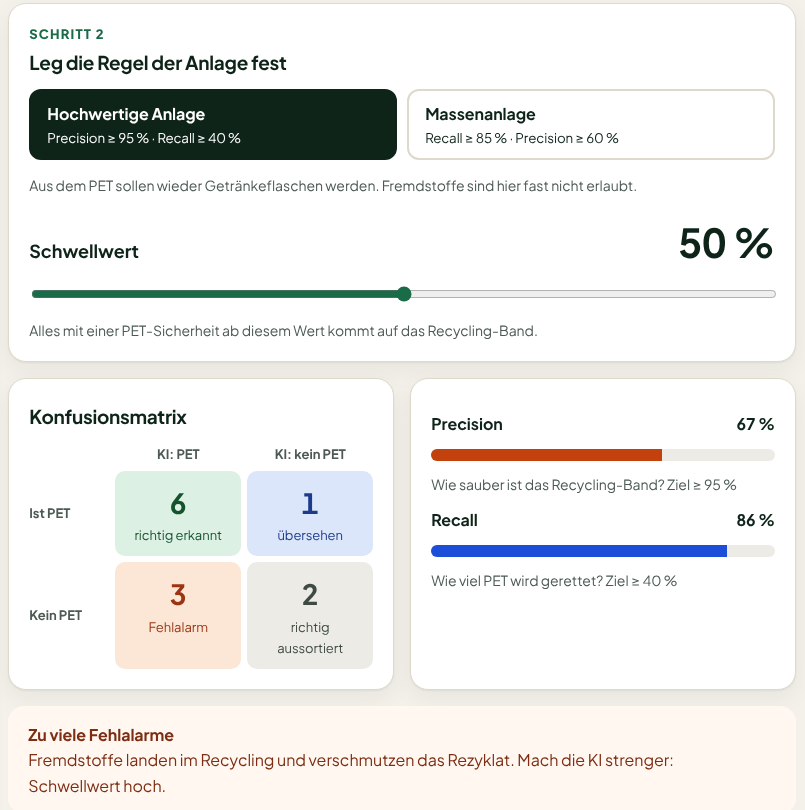
\includegraphics[width=\columnwidth]{fig/fig_line.png}
\caption{Modul 2 (Line Controller): Lernende setzen den Schwellwert der Sortier-KI und sehen Konfusionsmatrix, Precision und Recall unmittelbar (G1, G2, G4).}
\Description{Bildschirmfoto mit Schwellwert-Regler, Konfusionsmatrix und Balken für Precision und Recall.}
\label{fig:line}
\end{figure}

\begin{figure}[t]
\centering
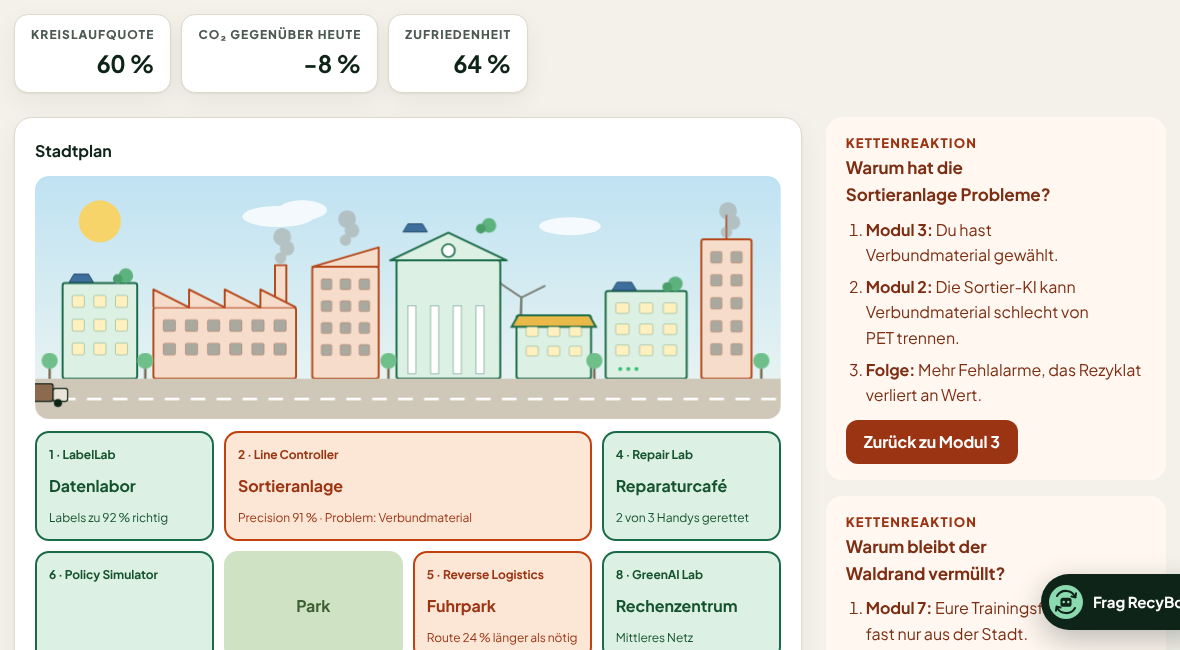
\includegraphics[width=\columnwidth]{fig/fig_capstone.png}
\caption{Modul 9 (Capstone): Die Ergebnisse aller Module werden zu Kennzahlen der Stadt verrechnet; Kettenreaktionen verbinden Module (G5).}
\Description{Bildschirmfoto mit Stadtplan, Kennzahlen und einer erklärten Kettenreaktion.}
\label{fig:capstone}
\end{figure}

\subsection{Umsetzung}
RecyBot 2.0 ist eine Webanwendung (React, TensorFlow.js) auf Deutsch und Englisch, die ohne Anmeldung im Browser läuft; Kamerabilder und Eingaben verlassen das Gerät nicht (A9). Die Bilderkennung nutzt Merkmalsvektoren des vortrainierten Netzes MobileNet \cite{howard2017} mit einer Nächste-Nachbarn-Klassifikation; Modul~4 lernt einen Entscheidungsbaum aus 48 Werkstattfällen \cite{quinlan1986}, Modul~5 nutzt eine Nächster-Nachbar-Heuristik mit 2-opt-Verbesserung \cite{applegate2006}, Modul~8 trainiert kleine neuronale Netze. Ein Bereich für Lehrkräfte erlaubt das Einbinden eines eigenen Teachable-Machine-Modells, das Verteilen eines vorkonfigurierten Links und die lokale Auswertung der Tests. Die Anwendung ist unter \url{https://recybot-projekt2.netlify.app} verfügbar, der Quellcode unter \repourl.

\section{Pilotstudie: Methode}
\label{sec:method}
\subsection{Design und Teilnehmende}
Die Pilotstudie war als explorative Eingruppen-Prä-/Post-Studie ohne Kontrollgruppe angelegt. Da eine Erhebung mit minderjährigen Schüler:innen die Zustimmung von Schulleitung und Erziehungsberechtigten erfordert, wurde im ersten Zyklus eine volljährige Gelegenheitsstichprobe als Stellvertretergruppe befragt. Teilgenommen haben $N = 11$ Personen (Median-Alter 22 Jahre, Spannweite 20--40), davon sechs Informatik-Studierende, eine Lehrkraft und vier Personen aus anderen Studiengängen bzw.\ Berufen. Das selbsteingeschätzte Vorwissen (1 = keins, 5 = sehr viel) lag für KI bei $M = 3.73$ ($SD = 0.90$) und für Kreislaufwirtschaft bei $M = 2.36$ ($SD = 1.21$).

\subsection{Instrumente}
\textit{Wissenstest:} sieben selbst entwickelte, nicht validierte Multiple-Choice-Items mit je vier Antwortoptionen zu LZ1 (Items 1, 5), LZ2 (Items 2--4) und LZ3 (Items 6, 7), identisch vor und nach der Nutzung; Summenwert 0--7. \textit{Usability:} System Usability Scale (SUS) in deutscher Fassung, zehn Items von 1 bis 5 \cite{brooke1996}. \textit{Spielerleben:} drei Items (Spaß, Interesse an den Inhalten, Einsatz im Unterricht bzw.\ Weiterempfehlung) von 1 bis 5. \textit{Offene Fragen:} Was hat gefallen, was war unverständlich, was sollte verbessert werden (freiwillig).

\subsection{Ablauf}
Die Erhebung fand im November 2026 online über ein Formular statt, ohne Aufsicht und auf eigenen Geräten (Dauer laut Information ca.\ 20--25 Minuten). Nach Information und Einwilligung folgten Angaben zur Person und der Wissenstest. Anschließend sollten die Teilnehmenden in einem neuen Tab die Module 1, 2, 4 und 7 spielen (ca.\ 10--15 Minuten) und die gespielten Module angeben. Danach folgten der Wissenstest erneut (mit der Bitte, nicht zurückzublättern), die SUS, die Items zum Spielerleben und die offenen Fragen.

\subsection{Auswertung}
Die Summenwerte vor und nach der Nutzung wurden mit einem zweiseitigen t-Test für abhängige Stichproben ($\alpha = .05$) verglichen; als Effektstärke wird $d_z$ (mittlere Differenz geteilt durch die Standardabweichung der Differenzen) berichtet. Wegen der kleinen Stichprobe und der diskreten Werte wurde zusätzlich ein Wilcoxon-Vorzeichen-Rang-Test gerechnet. Der SUS-Wert wurde nach Brooke \cite{brooke1996} berechnet. Die Auswertung erfolgte mit Python (pandas, SciPy); die von Skript und Formular berechneten Punktzahlen stimmen für alle Teilnehmenden überein.

\subsection{Ethik und Datenschutz}
Die Teilnehmenden wurden über Zweck, Dauer, Freiwilligkeit und Anonymität informiert und bestätigten, mindestens 18 Jahre alt und mit der anonymen Auswertung einverstanden zu sein. Es wurden keine Namen oder Kontaktdaten erhoben.
\section{Pilotstudie: Ergebnisse}
\label{sec:results}
\subsection{Nutzung}
Die Teilnehmenden spielten im Mittel 1.73 der vier vorgesehenen Module (Modul~1: $n = 6$, Modul~2: $n = 5$, Modul~4: $n = 3$, Modul~7: $n = 4$, weitere Module: $n = 1$); nur zwei Personen spielten alle vier.

\subsection{Wissenstest (FF2)}
Die mittlere Punktzahl stieg von $M = 2.73$ ($SD = 1.68$) auf $M = 3.27$ ($SD = 1.68$) von maximal 7 Punkten (Tabelle~\ref{tab:results}). Sechs Teilnehmende verbesserten sich, vier blieben gleich, eine Person verschlechterte sich. Der Zuwachs entspricht einem mittleren Effekt ($d_z = 0.67$), ist aber statistisch nicht signifikant ($t(10) = 2.21$, $p = .052$; Wilcoxon $p = .11$). Auf Itemebene stiegen die richtigen Antworten zu fehlerhaften Trainingsdaten (6 auf 8), zu Recall (4 auf 6) und zur Abfallhierarchie (1 auf 4); bei der Frage zur Reparatur sanken sie (5 auf 3).

\begin{table}[t]
\caption{Ergebnisse der Pilotstudie ($N = 11$)}
\label{tab:results}
\small
\begin{tabular}{@{}l r r@{}}
\toprule
\textbf{Wissenstest (richtige Antworten)} & \textbf{Prä} & \textbf{Post}\\
\midrule
1 Fehlerhafte Trainingsdaten (LZ1) & 6 & 8\\
2 Recall als Kennzahl (LZ2) & 4 & 6\\
3 Schwellwert und Precision (LZ2) & 5 & 6\\
4 Entscheidungsbaum (LZ2) & 4 & 4\\
5 Bias durch Klassenverteilung (LZ1) & 5 & 5\\
6 Abfallhierarchie (LZ3) & 1 & 4\\
7 Reparatur vor Recycling (LZ3) & 5 & 3\\
\midrule
Summenwert $M$ ($SD$), 0--7 & 2.73 (1.68) & 3.27 (1.68)\\
\multicolumn{3}{@{}l}{\footnotesize $t(10) = 2.21$, $p = .052$, $d_z = 0.67$; Wilcoxon: $p = .11$}\\
\midrule
\multicolumn{3}{@{}l}{\textbf{Nach der Nutzung}}\\
SUS $M$ ($SD$), 0--100 & \multicolumn{2}{r}{57.7 (19.1)}\\
Spaß $M$, 1--5 & \multicolumn{2}{r}{3.64}\\
Interesse an den Inhalten $M$, 1--5 & \multicolumn{2}{r}{3.82}\\
Unterrichtseinsatz / Empfehlung $M$, 1--5 & \multicolumn{2}{r}{3.64}\\
\bottomrule
\end{tabular}
\end{table}

\subsection{Usability und Spielerleben (FF3)}
Der SUS-Wert lag bei $M = 57.7$ ($SD = 19.1$; Spannweite 32.5--92.5) und damit unter dem Referenzwert von 68; nach der Adjektivskala von Bangor et al.\ entspricht er dem Bereich „OK“ \cite{bangor2009}. Spaß ($M = 3.64$), Interesse an den Inhalten ($M = 3.82$) und die Bereitschaft zum Einsatz bzw.\ zur Weiterempfehlung ($M = 3.64$) wurden moderat positiv bewertet. Die offenen Fragen beantworteten nur zwei Personen inhaltlich; genannt wurden die einfache Bedienung und die Verbindung von KI und Recycling als positiv, Fachbegriffe zu Beginn als Hürde sowie der Wunsch nach mehr praktischen Beispielen und kurzen Begriffserklärungen.

\section{Diskussion}
\label{sec:discussion}
\subsection{Gestaltung (FF1)}
Der Gestaltungsprozess zeigt, dass sich Lernziele, Inhalte und Spielmechaniken eines Lernspiels zu KI-Literacy und Kreislaufwirtschaft nachvollziehbar ableiten lassen: Jede Entscheidung ist auf eine Anforderung (Tabelle~\ref{tab:req}) oder ein Lernziel (Tabelle~\ref{tab:lz}) zurückgeführt, und das LM-GM-Modell macht explizit, welche Spielmechanik welche Lernmechanik trägt (Tabelle~\ref{tab:lmgm}). Gegenüber den Referenzsystemen übernimmt RecyBot bewusst das eigene Trainieren echter Modelle ohne Programmierung \cite{carney2020,codeorg2019}, erweitert es aber über Klassifikation hinaus und verankert es in einem Kreislauf, in dem Entscheidungen über KI und über Produkte, Reparatur und Politik aufeinander wirken. Die Prinzipien G1--G6 sind als Gestaltungsimplikationen auf andere Anwendungsfelder übertragbar, etwa auf Lernspiele zu KI in Gesundheit oder Mobilität. Einschränkend wurden die Kriterien K1--K4 vom Projektteam angewendet, ohne unabhängige Einschätzung; die Zuordnung von Modulen zu Lernzielen ist theoretisch begründet, aber nicht empirisch geprüft.

\subsection{Lernwirkung (FF2)}
Der beobachtete Zuwachs ist mittelgroß, aber nicht signifikant und bei $N = 11$ nicht belastbar. Er sollte zudem nicht als Wirkung des Gesamtkonzepts gelesen werden: Die Teilnehmenden spielten im Mittel weniger als die Hälfte der vorgesehenen Module und keines davon war Teil 2 oder das Capstone-Modul, sodass LZ4 und der rote Faden nicht erfasst wurden. Die Nutzung erfolgte unbegleitet und ohne unterrichtliche Einbettung, obwohl Lernspiele vor allem in Kombination mit weiterer Instruktion wirken \cite{wouters2013} und unangeleitete Exploration Noviz:innen überfordern kann \cite{kirschner2006}. Auf Itemebene stiegen die Antworten vor allem bei Konzepten, die in häufig gespielten Modulen direkt erfahrbar sind (Trainingsdaten in Modul~1, Recall in Modul~2). Der Anstieg bei der Abfallhierarchie lässt sich keinem gespielten Modul eindeutig zuordnen und kann auch auf die Testwiederholung zurückgehen; der Rückgang bei der Reparaturfrage betrifft ein Modul, das nur drei Personen spielten. Bei elf Personen und vier Antwortoptionen liegen Veränderungen um zwei Antworten zudem im Bereich zufälliger Schwankungen.

\subsection{Usability (FF3) und Folgerungen für den nächsten Zyklus}
Der SUS-Wert im Bereich „OK“ und die große Streuung deuten auf eine heterogene Nutzungserfahrung hin. Da die meisten Teilnehmenden nur ein bis zwei Module nutzten, spiegelt er vor allem den Einstieg wider; die Rückmeldung zu Fachbegriffen passt dazu. Für den nächsten DBR-Zyklus ergeben sich vier Änderungen: (1) ein kurzes Onboarding vor jedem Modul, (2) im Text eingebundene Begriffserklärungen statt eines separaten Glossars, um die extrinsische Belastung zu senken \cite{mayer2009}, (3) die Zuordnung der zwölf integrierten Testaufgaben zu LZ1--LZ4 einschließlich Transferaufgaben und ihre Pilotierung und (4) eine Erprobung im begleiteten Unterricht statt unbeaufsichtigt.

\subsection{Limitationen}
Die Literaturübersicht ist narrativ; ohne Trefferdokumentation können relevante Arbeiten fehlen, und viele Befunde stammen aus anderen Zielgruppen. Der Vergleich mit Referenzsystemen beruht auf veröffentlichten Beschreibungen und umfasst eine Auswahl. Die Pilotstudie umfasst eine kleine, volljährige Gelegenheitsstichprobe mit überdurchschnittlichem KI-Vorwissen statt der Zielgruppe, keine Kontrollgruppe und einen nicht validierten Test mit sieben Items, dessen Wiederholung Erinnerungseffekte begünstigt. Einzelne Inhalte beruhen auf Vereinfachungen (simulierte Sensordaten und geschätzter Energieverbrauch in Modul~8, regelbasierte Stadtkennzahlen in Modul~9).

\subsection{Geplante Hauptstudie}
Geplant ist eine quasi-experimentelle Studie mit Wartekontrollgruppe und drei Messzeitpunkten (vor, direkt nach und drei Wochen nach der Nutzung) in ganzen Klassen, getrennt nach Sekundarstufe~I (Jahrgangsstufen 9--10) und Sekundarstufe~II, mit je zwei Versuchs- und zwei Kontrollklassen. Eine a-priori-Poweranalyse für die Interaktion Messzeitpunkt $\times$ Gruppe (Varianzanalyse mit Messwiederholung; $f = 0.25$ \cite{cohen1988}, $\alpha = .05$, $1-\beta = .80$, $r = .50$) ergibt eine Mindeststichprobe von $N = 28$ je Teilstichprobe; vier Klassen (ca.\ 100 Lernende) berücksichtigen Klassenstruktur und Ausfälle. Erhoben werden konzeptuelles Wissen, Transfer, Usability, kognitive Belastung \cite{klepsch2017} und Spielerleben; Voraussetzung sind die Genehmigung der Schulleitung und die Einwilligung der Erziehungsberechtigten.

\section{Fazit}
RecyBot 2.0 verbindet KI-Literacy und Kreislaufwirtschaft in einem Lernspiel, dessen Lernziele, Inhalte und Spielmechaniken nachvollziehbar aus Kompetenzrahmen, Lerntheorien und Referenzsystemen abgeleitet sind (FF1). Die explorative Pilotstudie liefert erste, nicht signifikante Hinweise auf einen Wissenszuwachs (FF2) und zeigt Überarbeitungsbedarf bei Einstieg und Begriffsklärung (FF3). Die abgeleiteten Gestaltungsprinzipien und die offen verfügbaren Materialien sollen die Weiterentwicklung und eine Überprüfung mit der eigentlichen Zielgruppe ermöglichen.

\section*{Verfügbarkeit von Daten und Materialien}
Quellcode der Anwendung, vollständiger Fragebogen mit Lösungen, Einwilligungstext, Ablaufbeschreibung, Rohdaten, Codebuch und Auswertungsskript sind unter \repourl{} verfügbar. Das Skript reproduziert alle in Abschnitt~\ref{sec:results} berichteten Kennwerte.

\section*{Hinweis zur Nutzung von KI-Werkzeugen}
Die Anwendung RecyBot 2.0 wurde zu einem großen Teil mit dem KI-Assistenten Claude (Anthropic) programmiert. Lernkonzept, Lernziele, didaktische Begründungen und die Erprobung lagen beim Projektteam. Textentwürfe, die statistische Auswertung und die Formatierung dieses Papers wurden mit Claude erstellt; die vorliegende Fassung wurde mit Claude auf Grundlage der Rückmeldungen der Betreuerin umstrukturiert. Grundlage waren stets die Vorgaben, Daten und Rückmeldungen des Projektteams, das alle Inhalte geprüft hat und verantwortet. Die vollständigen Prompts, einschließlich derer zur Literaturrecherche, liegen im genannten Repository.
\begin{thebibliography}{52}
\small
\bibitem{amershi2014} Saleema Amershi, Maya Cakmak, W. Bradley Knox, and Todd Kulesza. 2014. Power to the People: The Role of Humans in Interactive Machine Learning. \textit{AI Magazine} 35, 4, 105--120.
\bibitem{anderson2001} Lorin W. Anderson and David R. Krathwohl (Eds.). 2001. \textit{A Taxonomy for Learning, Teaching, and Assessing: A Revision of Bloom's Taxonomy of Educational Objectives}. Longman, New York.
\bibitem{applegate2006} David L. Applegate, Robert E. Bixby, Vašek Chvátal, and William J. Cook. 2006. \textit{The Traveling Salesman Problem: A Computational Study}. Princeton University Press.
\bibitem{arnab2015} Sylvester Arnab, Theodore Lim, Maira B. Carvalho, Francesco Bellotti, Sara de Freitas, Sandy Louchart, Neil Suttie, Riccardo Berta, and Alessandro De Gloria. 2015. Mapping Learning and Game Mechanics for Serious Games Analysis. \textit{British Journal of Educational Technology} 46, 2, 391--411.
\bibitem{bangor2009} Aaron Bangor, Philip Kortum, and James Miller. 2009. Determining What Individual SUS Scores Mean: Adding an Adjective Rating Scale. \textit{Journal of Usability Studies} 4, 3, 114--123.
\bibitem{biggs2011} John Biggs and Catherine Tang. 2011. \textit{Teaching for Quality Learning at University} (4th ed.). Open University Press, Maidenhead.
\bibitem{bocken2016} Nancy M. P. Bocken, Ingrid de Pauw, Conny Bakker, and Bram van der Grinten. 2016. Product Design and Business Model Strategies for a Circular Economy. \textit{Journal of Industrial and Production Engineering} 33, 5, 308--320.
\bibitem{brooke1996} John Brooke. 1996. SUS: A „Quick and Dirty“ Usability Scale. In \textit{Usability Evaluation in Industry}, Patrick W. Jordan et al.\ (Eds.). Taylor \& Francis, London, 189--194.
\bibitem{carney2020} Michelle Carney, Barron Webster, Irene Alvarado, Kyle Phillips, Noura Howell, Jordan Griffith, Jonas Jongejan, Amit Pitaru, and Alexander Chen. 2020. Teachable Machine: Approachable Web-Based Tool for Exploring Machine Learning Classification. In \textit{Extended Abstracts of the 2020 CHI Conference on Human Factors in Computing Systems}. ACM.
\bibitem{codeorg2019} Code.org. 2019. AI for Oceans. Online-Lernaktivität. \url{https://code.org/oceans}
\bibitem{ctgv1990} Cognition and Technology Group at Vanderbilt. 1990. Anchored Instruction and Its Relationship to Situated Cognition. \textit{Educational Researcher} 19, 6, 2--10.
\bibitem{cohen1988} Jacob Cohen. 1988. \textit{Statistical Power Analysis for the Behavioral Sciences} (2nd ed.). Lawrence Erlbaum, Hillsdale, NJ.
\bibitem{dbrc2003} Design-Based Research Collective. 2003. Design-Based Research: An Emerging Paradigm for Educational Inquiry. \textit{Educational Researcher} 32, 1, 5--8.
\bibitem{druga2019} Stefania Druga, Sarah T. Vu, Eesh Likhith, and Tammy Qiu. 2019. Inclusive AI Literacy for Kids around the World. In \textit{Proceedings of FabLearn 2019}. ACM.
\bibitem{emf2013} Ellen MacArthur Foundation. 2013. \textit{Towards the Circular Economy, Vol. 1: Economic and Business Rationale for an Accelerated Transition}.
\bibitem{eu2020} Europäische Kommission. 2020. \textit{Ein neuer Aktionsplan für die Kreislaufwirtschaft: Für ein saubereres und wettbewerbsfähigeres Europa}. COM(2020) 98 final.
\bibitem{fawcett2006} Tom Fawcett. 2006. An Introduction to ROC Analysis. \textit{Pattern Recognition Letters} 27, 8, 861--874.
\bibitem{hamari2014} Juho Hamari, Jonna Koivisto, and Harri Sarsa. 2014. Does Gamification Work? A Literature Review of Empirical Studies on Gamification. In \textit{Proceedings of the 47th Hawaii International Conference on System Sciences}. IEEE.
\bibitem{hanus2015} Michael D. Hanus and Jesse Fox. 2015. Assessing the Effects of Gamification in the Classroom. \textit{Computers \& Education} 80, 152--161.
\bibitem{hattie2007} John Hattie and Helen Timperley. 2007. The Power of Feedback. \textit{Review of Educational Research} 77, 1, 81--112.
\bibitem{howard2017} Andrew G. Howard, Menglong Zhu, Bo Chen, Dmitry Kalenichenko, Weijun Wang, Tobias Weyand, Marco Andreetto, and Hartwig Adam. 2017. MobileNets: Efficient Convolutional Neural Networks for Mobile Vision Applications. arXiv:1704.04861.
\bibitem{kapur2008} Manu Kapur. 2008. Productive Failure. \textit{Cognition and Instruction} 26, 3, 379--424.
\bibitem{kirchherr2017} Julian Kirchherr, Denise Reike, and Marko Hekkert. 2017. Conceptualizing the Circular Economy: An Analysis of 114 Definitions. \textit{Resources, Conservation and Recycling} 127, 221--232.
\bibitem{kirschner2006} Paul A. Kirschner, John Sweller, and Richard E. Clark. 2006. Why Minimal Guidance During Instruction Does Not Work. \textit{Educational Psychologist} 41, 2, 75--86.
\bibitem{klepsch2017} Melina Klepsch, Florian Schmitz, and Tina Seufert. 2017. Development and Validation of Two Instruments Measuring Intrinsic, Extraneous, and Germane Cognitive Load. \textit{Frontiers in Psychology} 8, 1997.
\bibitem{kmk2016} Kultusministerkonferenz. 2016. \textit{Bildung in der digitalen Welt: Strategie der Kultusministerkonferenz}. Berlin.
\bibitem{kolb1984} David A. Kolb. 1984. \textit{Experiential Learning: Experience as the Source of Learning and Development}. Prentice-Hall, Englewood Cliffs, NJ.
\bibitem{lane2021} Dale Lane. 2021. \textit{Machine Learning for Kids: A Project-Based Introduction to Artificial Intelligence}. No Starch Press, San Francisco.
\bibitem{lange2022} Kim P. H. Lange, Gijsbert Korevaar, Inge F. Oskam, and Paulien M. Herder. 2022. Re-Organise: Game-Based Learning of Circular Business Model Innovation. \textit{Frontiers in Sustainability} 3, 809700.
\bibitem{long2020} Duri Long and Brian Magerko. 2020. What Is AI Literacy? Competencies and Design Considerations. In \textit{Proceedings of the 2020 CHI Conference on Human Factors in Computing Systems}. ACM.
\bibitem{mayer2009} Richard E. Mayer. 2009. \textit{Multimedia Learning} (2nd ed.). Cambridge University Press.
\bibitem{mayer2019} Richard E. Mayer. 2019. Computer Games in Education. \textit{Annual Review of Psychology} 70, 531--549.
\bibitem{meadows2008} Donella H. Meadows. 2008. \textit{Thinking in Systems: A Primer}. Chelsea Green Publishing, White River Junction, VT.
\bibitem{unesco2024} Fengchun Miao and Kelly Shiohira. 2024. \textit{AI Competency Framework for Students}. UNESCO, Paris.
\bibitem{paas2010} Fred Paas, Tamara van Gog, and John Sweller. 2010. Cognitive Load Theory: New Conceptualizations, Specifications, and Integrated Research Perspectives. \textit{Educational Psychology Review} 22, 115--121.
\bibitem{perkins1992} David N. Perkins and Gavriel Salomon. 1992. Transfer of Learning. In \textit{International Encyclopedia of Education} (2nd ed.). Pergamon Press, Oxford.
\bibitem{plass2015} Jan L. Plass, Bruce D. Homer, and Charles K. Kinzer. 2015. Foundations of Game-Based Learning. \textit{Educational Psychologist} 50, 4, 258--283.
\bibitem{quinlan1986} J. Ross Quinlan. 1986. Induction of Decision Trees. \textit{Machine Learning} 1, 1, 81--106.
\bibitem{rowe2011} Jonathan P. Rowe, Lucy R. Shores, Bradford W. Mott, and James C. Lester. 2011. Integrating Learning, Problem Solving, and Engagement in Narrative-Centered Learning Environments. \textit{International Journal of Artificial Intelligence in Education} 21, 115--133.
\bibitem{sambasivan2021} Nithya Sambasivan, Shivani Kapania, Hannah Highfill, Diana Akrong, Praveen Paritosh, and Lora M. Aroyo. 2021. „Everyone Wants to Do the Model Work, Not the Data Work“: Data Cascades in High-Stakes AI. In \textit{Proceedings of the 2021 CHI Conference on Human Factors in Computing Systems}. ACM.
\bibitem{schwartz2020} Roy Schwartz, Jesse Dodge, Noah A. Smith, and Oren Etzioni. 2020. Green AI. \textit{Communications of the ACM} 63, 12, 54--63.
\bibitem{shneiderman1983} Ben Shneiderman. 1983. Direct Manipulation: A Step Beyond Programming Languages. \textit{Computer} 16, 8, 57--69.
\bibitem{shute2008} Valerie J. Shute. 2008. Focus on Formative Feedback. \textit{Review of Educational Research} 78, 1, 153--189.
\bibitem{stahel2013} Walter R. Stahel. 2013. Policy for Material Efficiency: Sustainable Taxation as a Departure from the Throwaway Society. \textit{Philosophical Transactions of the Royal Society A} 371.
\bibitem{sterman2000} John D. Sterman. 2000. \textit{Business Dynamics: Systems Thinking and Modeling for a Complex World}. McGraw-Hill, Boston.
\bibitem{strubell2019} Emma Strubell, Ananya Ganesh, and Andrew McCallum. 2019. Energy and Policy Considerations for Deep Learning in NLP. In \textit{Proceedings of the 57th Annual Meeting of the Association for Computational Linguistics}.
\bibitem{sweller1988} John Sweller. 1988. Cognitive Load During Problem Solving: Effects on Learning. \textit{Cognitive Science} 12, 2, 257--285.
\bibitem{touretzky2019} David Touretzky, Christina Gardner-McCune, Fred Martin, and Deborah Seehorn. 2019. Envisioning AI for K-12: What Should Every Child Know about AI? In \textit{Proceedings of the AAAI Conference on Artificial Intelligence}.
\bibitem{vanroy2019} Rob van Roy and Bieke Zaman. 2019. Unravelling the Ambivalent Motivational Power of Gamification: A Basic Psychological Needs Perspective. \textit{International Journal of Human-Computer Studies} 127, 38--50.
\bibitem{wiek2011} Arnim Wiek, Lauren Withycombe, and Charles L. Redman. 2011. Key Competencies in Sustainability: A Reference Framework for Academic Program Development. \textit{Sustainability Science} 6, 2, 203--218.
\bibitem{wouters2013} Pieter Wouters, Christof van Nimwegen, Herre van Oostendorp, and Erik D. van der Spek. 2013. A Meta-Analysis of the Cognitive and Motivational Effects of Serious Games. \textit{Journal of Educational Psychology} 105, 2, 249--265.
\bibitem{zheng2017} Nan-ning Zheng et al. 2017. Hybrid-Augmented Intelligence: Collaboration and Cognition. \textit{Frontiers of Information Technology \& Electronic Engineering} 18, 2, 153--179.
\end{thebibliography}
\end{document}
